 \documentclass[12pt]{amsart}
% packages
\usepackage{graphicx}
\usepackage{setspace}
\usepackage{amssymb,amsmath,amsthm,amsfonts,amscd}
\usepackage{hyperref}
\usepackage{color}
\usepackage{booktabs}
\usepackage{tabularx}
\usepackage{enumitem}
\usepackage[retainorgcmds]{IEEEtrantools}
\usepackage[notref,notcite,final]{showkeys}
\usepackage[final]{pdfpages}
\usepackage{fancyhdr}
\usepackage{upgreek}
\usepackage{multicol}
\usepackage{mathtools}

\usepackage{fancyvrb}
\usepackage{listings}
% set margin as 0.75in
\usepackage[margin=0.75in]{geometry}

% tikz-related settings
\usepackage{tikz}
\usepackage{tikz-cd}
\usetikzlibrary{cd}

% theorem environments with italic font
\newtheorem{thm}{Theorem}[section]
\newtheorem*{thm*}{Theorem}
\newtheorem{lemma}[thm]{Lemma}
\newtheorem{prop}[thm]{Proposition}
\newtheorem{claim}[thm]{Claim}
\newtheorem{corollary}[thm]{Corollary}
\newtheorem{conjecture}[thm]{Conjecture}
\newtheorem{question}[thm]{Question}
\newtheorem{procedure}[thm]{Procedure}
\newtheorem{assumption}[thm]{Assumption}

% theorem environments with roman font (use lower-case version in body
% of text, e.g., \begin{example} rather than \begin{Example})
\newtheorem{Definition}[thm]{Definition}
\newenvironment{definition}
{\begin{Definition}\rm}{\end{Definition}}
\newtheorem{Example}[thm]{Example}
\newenvironment{example}
{\begin{Example}\rm}{\end{Example}}

\theoremstyle{definition}
\newtheorem{remark}[thm]{\textbf{Remark}}

% special sets
\newcommand{\A}{\mathbb{A}}
\newcommand{\C}{\mathbb{C}}
\newcommand{\F}{\mathbb{F}}
\newcommand{\N}{\mathbb{N}}
\newcommand{\Q}{\mathbb{Q}}
\newcommand{\R}{\mathbb{R}}
\newcommand{\Z}{\mathbb{Z}}
\newcommand{\cals}{\mathcal{S}}
\newcommand{\ZZ}{\mathbb{Z}_{\ge 0}}
\newcommand{\cala}{\mathcal{A}}
\newcommand{\calb}{\mathcal{B}}
\newcommand{\cald}{\mathcal{D}}
\newcommand{\calh}{\mathcal{H}}
\newcommand{\call}{\mathcal{L}}
\newcommand{\calr}{\mathcal{R}}
\newcommand{\la}{\mathbf{a}}
\newcommand{\lgl}{\mathfrak{gl}}
\newcommand{\lsl}{\mathfrak{sl}}
\newcommand{\lieg}{\mathfrak{g}}

% math operators
\DeclareMathOperator{\kernel}{\mathrm{ker}}
\DeclareMathOperator{\image}{\mathrm{im}}
\DeclareMathOperator{\rad}{\mathrm{rad}}
\DeclareMathOperator{\id}{\mathrm{id}}
\DeclareMathOperator{\hum}{[\mathrm{Hum}]}
\DeclareMathOperator{\eh}{[\mathrm{EH}]}
\DeclareMathOperator{\lcm}{\mathrm{lcm}}
\DeclareMathOperator{\Aut}{\mathrm{Aut}}
\DeclareMathOperator{\Inn}{\mathrm{Inn}}
\DeclareMathOperator{\Out}{\mathrm{Out}}
\DeclareMathOperator{\Gal}{\mathrm{Gal}}


% frequently used shorthands
\newcommand{\ra}{\rightarrow}
\newcommand{\se}{\subseteq}
\newcommand{\ip}[1]{\langle#1\rangle}
\newcommand{\dual}{^*}
\newcommand{\inverse}{^{-1}}
\newcommand{\norm}[2]{\|#1\|_{#2}}
\newcommand{\abs}[1]{\lvert #1 \rvert}
\newcommand{\Abs}[1]{\bigg| #1 \bigg|}
\newcommand\bm[1]{\begin{bmatrix}#1\end{bmatrix}}
\newcommand{\op}{\text{op}}

% nicer looking empty set
\let\oldemptyset\emptyset
\let\emptyset\varnothing

\setlist[enumerate,1]{topsep=1em,leftmargin=1.8em, itemsep=0.5em, label=\textup{(}\arabic*\textup{)}}
\setlist[enumerate,2]{topsep=0.5em,leftmargin=3em, itemsep=0.3em}

%pagestyle
%\pagestyle{fancy} 

\begin{document}
\begin{center}
    \textsc{Random Walks. HW 5\\ Ian Jorquera\\ Collaboration: Tristan, Alex}
\end{center}
\vspace{1em}


\definecolor{codegreen}{rgb}{0,0.6,0}
\definecolor{codegray}{rgb}{0.5,0.5,0.5}
\definecolor{codepurple}{rgb}{0.58,0,0.82}
\definecolor{backcolour}{rgb}{1,1,1}

\lstdefinestyle{mystyle}{
    backgroundcolor=\color{backcolour},   
    commentstyle=\color{codegray},
    keywordstyle=\color{magenta},
    numberstyle=\tiny\color{codegray},
    stringstyle=\color{codegreen},
    basicstyle=\ttfamily\footnotesize,
    breakatwhitespace=false,         
    breaklines=true,                 
    captionpos=b,                    
    keepspaces=true,                 
    numbers=left,                    
    numbersep=5pt,                  
    showspaces=false,                
    showstringspaces=false,
    showtabs=false,                  
    tabsize=2
}

\lstset{style=mystyle}


\begin{enumerate}
    \item I've taken much of the work for this problem from the previous quiz(which i completed with the collaborators listed above). Consider the fractional derivative $\prescript{}{0}{D}^{\nu}_{x} x^\mu=\frac{d^n}{dx^n}\prescript{}{0}{I}^{n-\nu}_{x}x^\mu$ where $n=\lfloor\nu\rfloor+1$.

    \begin{align*}
        \frac{d^n}{dx^n}\prescript{}{0}{I}^{n-\nu}_{x}x^\mu &= \frac{1}{\Gamma(n-\nu-1)}\frac{d^n}{dx^n}\int_{0}^x t^\mu(x-t)^{n-\nu-1}\,dt\\
    \end{align*}
    And let $u=\frac{t}{x}$ and $du=\frac{dt}{x}$ and we have that
    \begin{align*}
        &= \frac{1}{\Gamma(n-\nu)}\frac{d^n}{dx^n}\int_{0}^1 (xu)^\mu(x-xu)^{n-\nu-1}x\,du\\
        &= \frac{1}{\Gamma(n-\nu)}\frac{d^n}{dx^n}\int_{0}^1 x^\mu x^{n-\nu-1}x u^\mu (1-u)^{n-\nu-1}\,du\\
        &= \frac{1}{\Gamma(n-\nu)}\frac{d^n}{dx^n}x^{n-\nu+\mu}\int_{0}^1 u^\mu (1-u)^{n-\nu-1}\,du\\
    \end{align*}
    And with the definition of the beta function we have that 
    \begin{align*}
        &= \frac{1}{\Gamma(n-\nu)}\frac{d^n}{dx^n}x^{n-\nu+\mu}\frac{\Gamma(\mu+1)\Gamma(n-\nu)}{\Gamma(\mu-\nu+n+1)}\\
        &= \frac{1}{\Gamma(n-\nu)}\frac{\Gamma(\mu+1)\Gamma(n-\nu)\Gamma(n-\nu+\mu+1)}{\Gamma(\mu-\nu+n+1)\Gamma(\mu-\nu+1)} x^{\mu-\nu}\\
        &= \frac{\Gamma(\mu+1)}{\Gamma(\mu-\nu+1)} x^{\mu-\nu}\\ 
    \end{align*}

    \item First we will apply the Laplace transform of the fractional derivative on the function $f(x)$
    \begin{align*}
        \mathcal{L}\left\{\frac{d^n}{dx^n}\prescript{}{0}{I}^{n-\nu}_{x}f(x)\right\} &= \frac{1}{\Gamma(n-\nu)}\mathcal{L}\left\{\frac{d^n}{dx^n}\int_{0}^x f(t)(x-t)^{n-\nu-1}\,dt\right\}\\
        &=\frac{1}{\Gamma(n-\nu)}s^n\mathcal{L}\left\{\int_{0}^x f(t)(x-t)^{n-\nu-1}\,dt\right\}-\sum_{i=2}^n s^{n-i}\frac{d^{i-1}}{d x^{i-1}} \int_{0}^x f(t)(x-t)^{n-\nu-1}\,dt\Big\vert_{x=0}\\
        &=\frac{1}{\Gamma(n-\nu)}s^n f(s)\mathcal{L}\left\{x^{n-\nu-1}\right\}-\dots\\
        &=s^n f(s)s^{-n+\nu} -\dots \\
        &= s^\nu f(s) -\frac{1}{\Gamma(n-\nu)}\sum_{i=2}^n s^{n-i}\frac{d^{i-1}}{d x^{i-1}} \int_{0}^x f(t)(x-t)^{n-\nu-1}\,dt\Big\vert_{x=0}
    \end{align*}
    The second to last step follows from the Tauberian theorem with $\rho=n-\nu$. %spell check needed for red underline

    \item To solve this Fokker-Planck equation
    $$\frac{\partial p(x,t)}{\partial t}=D\frac{\partial^2 p(x,t)}{\partial x^2}- v\frac{\partial p(x,t)}{\partial x}$$
    We will first take the Laplace transform, and know that $p(x,0)=\delta(x)$, we get 

    \begin{align*}
        sp(x,s)-\delta(x)=D\frac{\partial^2 p(x,s)}{\partial x^2}- v\frac{\partial p(x,s)}{\partial x}
    \end{align*}
    We can then take the Fourier transform and get that

    \begin{align*}
        sp(k,s)-1&=D (ik)^2 p(k,s)- v(ik)p(k,s)\\
        p(k,s)&=\frac{1}{s+Dk^2+vik}\\
    \end{align*}
    And then taking the inverse Laplace transform we find that % https://en.wikipedia.org/wiki/Characteristic_function_(probability_theory)
    \begin{align*}
        p(k,t)&=\text{exp}(-vtik-Dtk^2)\\
    \end{align*}
    And finally with an inverse Fourier transform we find that   
    \begin{align*}
        p(k,t)&=\text{exp}(-vtik-Dtk^2)=\text{exp}(-ik vt-\frac{1}{2}(\sqrt{2Dt})^2k^2)\\  % mu = vt and sigma = \sqrt{2Dt}
        p(x,t) &= \frac{1}{\sqrt{4\pi D t}}\,\text{exp}\left( -\frac{\left(x-vt\right)^2}{4Dt}\right)
    \end{align*}

    \item The fractional derivative is as follows
    \begin{align*}
        \prescript{}{0}{D}^{\frac{1}{2}}_{t}\text{exp}(t) &= \prescript{}{0}{D}^{\frac{1}{2}}_{t}\sum_{n=0}^{\infty}\frac{x^n}{\Gamma(n+1)}\\
        &= \sum_{n=0}^{\infty}\frac{\prescript{}{0}{D}^{\frac{1}{2}}_{t}x^n}{\Gamma(n+1)}\\
        &= \sum_{n=0}^{\infty}\frac{\Gamma(n+1)x^{n-\frac{1}{2}}}{\Gamma(n+\frac{1}{2})\Gamma(n+1)}\\
        &= x^{-\frac{1}{2}}\sum_{n=0}^{\infty}\frac{x^{n}}{\Gamma(-\frac{1}{2}+n+1)}\\
    \end{align*}
    And from \href{https://en.wikipedia.org/wiki/Incomplete_gamma_function}{this} Wikipedia page under Holomorphic extension we know that 
    \begin{align*}
        &= e^{x}\frac{\gamma(-\frac{1}{2},x)}{\Gamma(-\frac{1}{2})}
    \end{align*}


    \item To see that $P(x,t)\propto \text{exp}\left(-\frac{\mu_\alpha U(x)}{K_\alpha}\right)$ is a steady state solution notice that 
        $$\prescript{}{0}{D}^{1-\alpha}_{t} \frac{\partial}{\partial x}\left[-\mu_\alpha \left(-\frac{\partial U(x)}{\partial x}\right) \text{exp}\left(-\frac{\mu_\alpha U(x)}{K_\alpha}\right)+K_\alpha \frac{\partial}{\partial x}\text{exp}\left(-\frac{\mu_\alpha U(x)}{K_\alpha}\right)\right]$$
        $$\prescript{}{0}{D}^{1-\alpha}_{t} \frac{\partial}{\partial x}\left[\mu_\alpha \frac{\partial U(x)}{\partial x} \text{exp}\left(-\frac{\mu_\alpha U(x)}{K_\alpha}\right)-K_\alpha \frac{\partial U(x)}{\partial x}\frac{\mu_\alpha }{K_\alpha}\text{exp}\left(-\frac{\mu_\alpha U(x)}{K_\alpha}\right)\right]$$
        $$\prescript{}{0}{D}^{1-\alpha}_{t} \frac{\partial}{\partial x}\left[\mu_\alpha \frac{\partial U(x)}{\partial x} \text{exp}\left(-\frac{\mu_\alpha U(x)}{K_\alpha}\right)-\mu_\alpha\frac{\partial U(x)}{\partial x} \text{exp}\left(-\frac{\mu_\alpha U(x)}{K_\alpha}\right)\right]$$
        $$\prescript{}{0}{D}^{1-\alpha}_{t} \frac{\partial}{\partial x}\left[0\right]$$
        $$\prescript{}{0}{D}^{1-\alpha}_{t}0=0$$
        And so $P(x,t)\propto \text{exp}\left(-\frac{\mu_\alpha U(x)}{K_\alpha}\right)$ is a steady state solution

    \item In the zeroth iteration of the generation of this fractal, where there is just a single filled in square the length is $L_0$ and the mass is $M_0$. In the first iteration the length is then $3L_0$ and the mass is $5M_0$. And because we know that $L^{d_f}\sim M$ we know that $d_f=\frac{\log(5)}{\log(3)}$. We can then find the spectral dimension and the dimension of the walk by first finding the resistance of the fractal. This can be done by building a resistor network for the zeroth iteration and the first iteration and comparing the increase in resistance with respect to length. work for this problem is shown on the next page.
    \newpage
    
    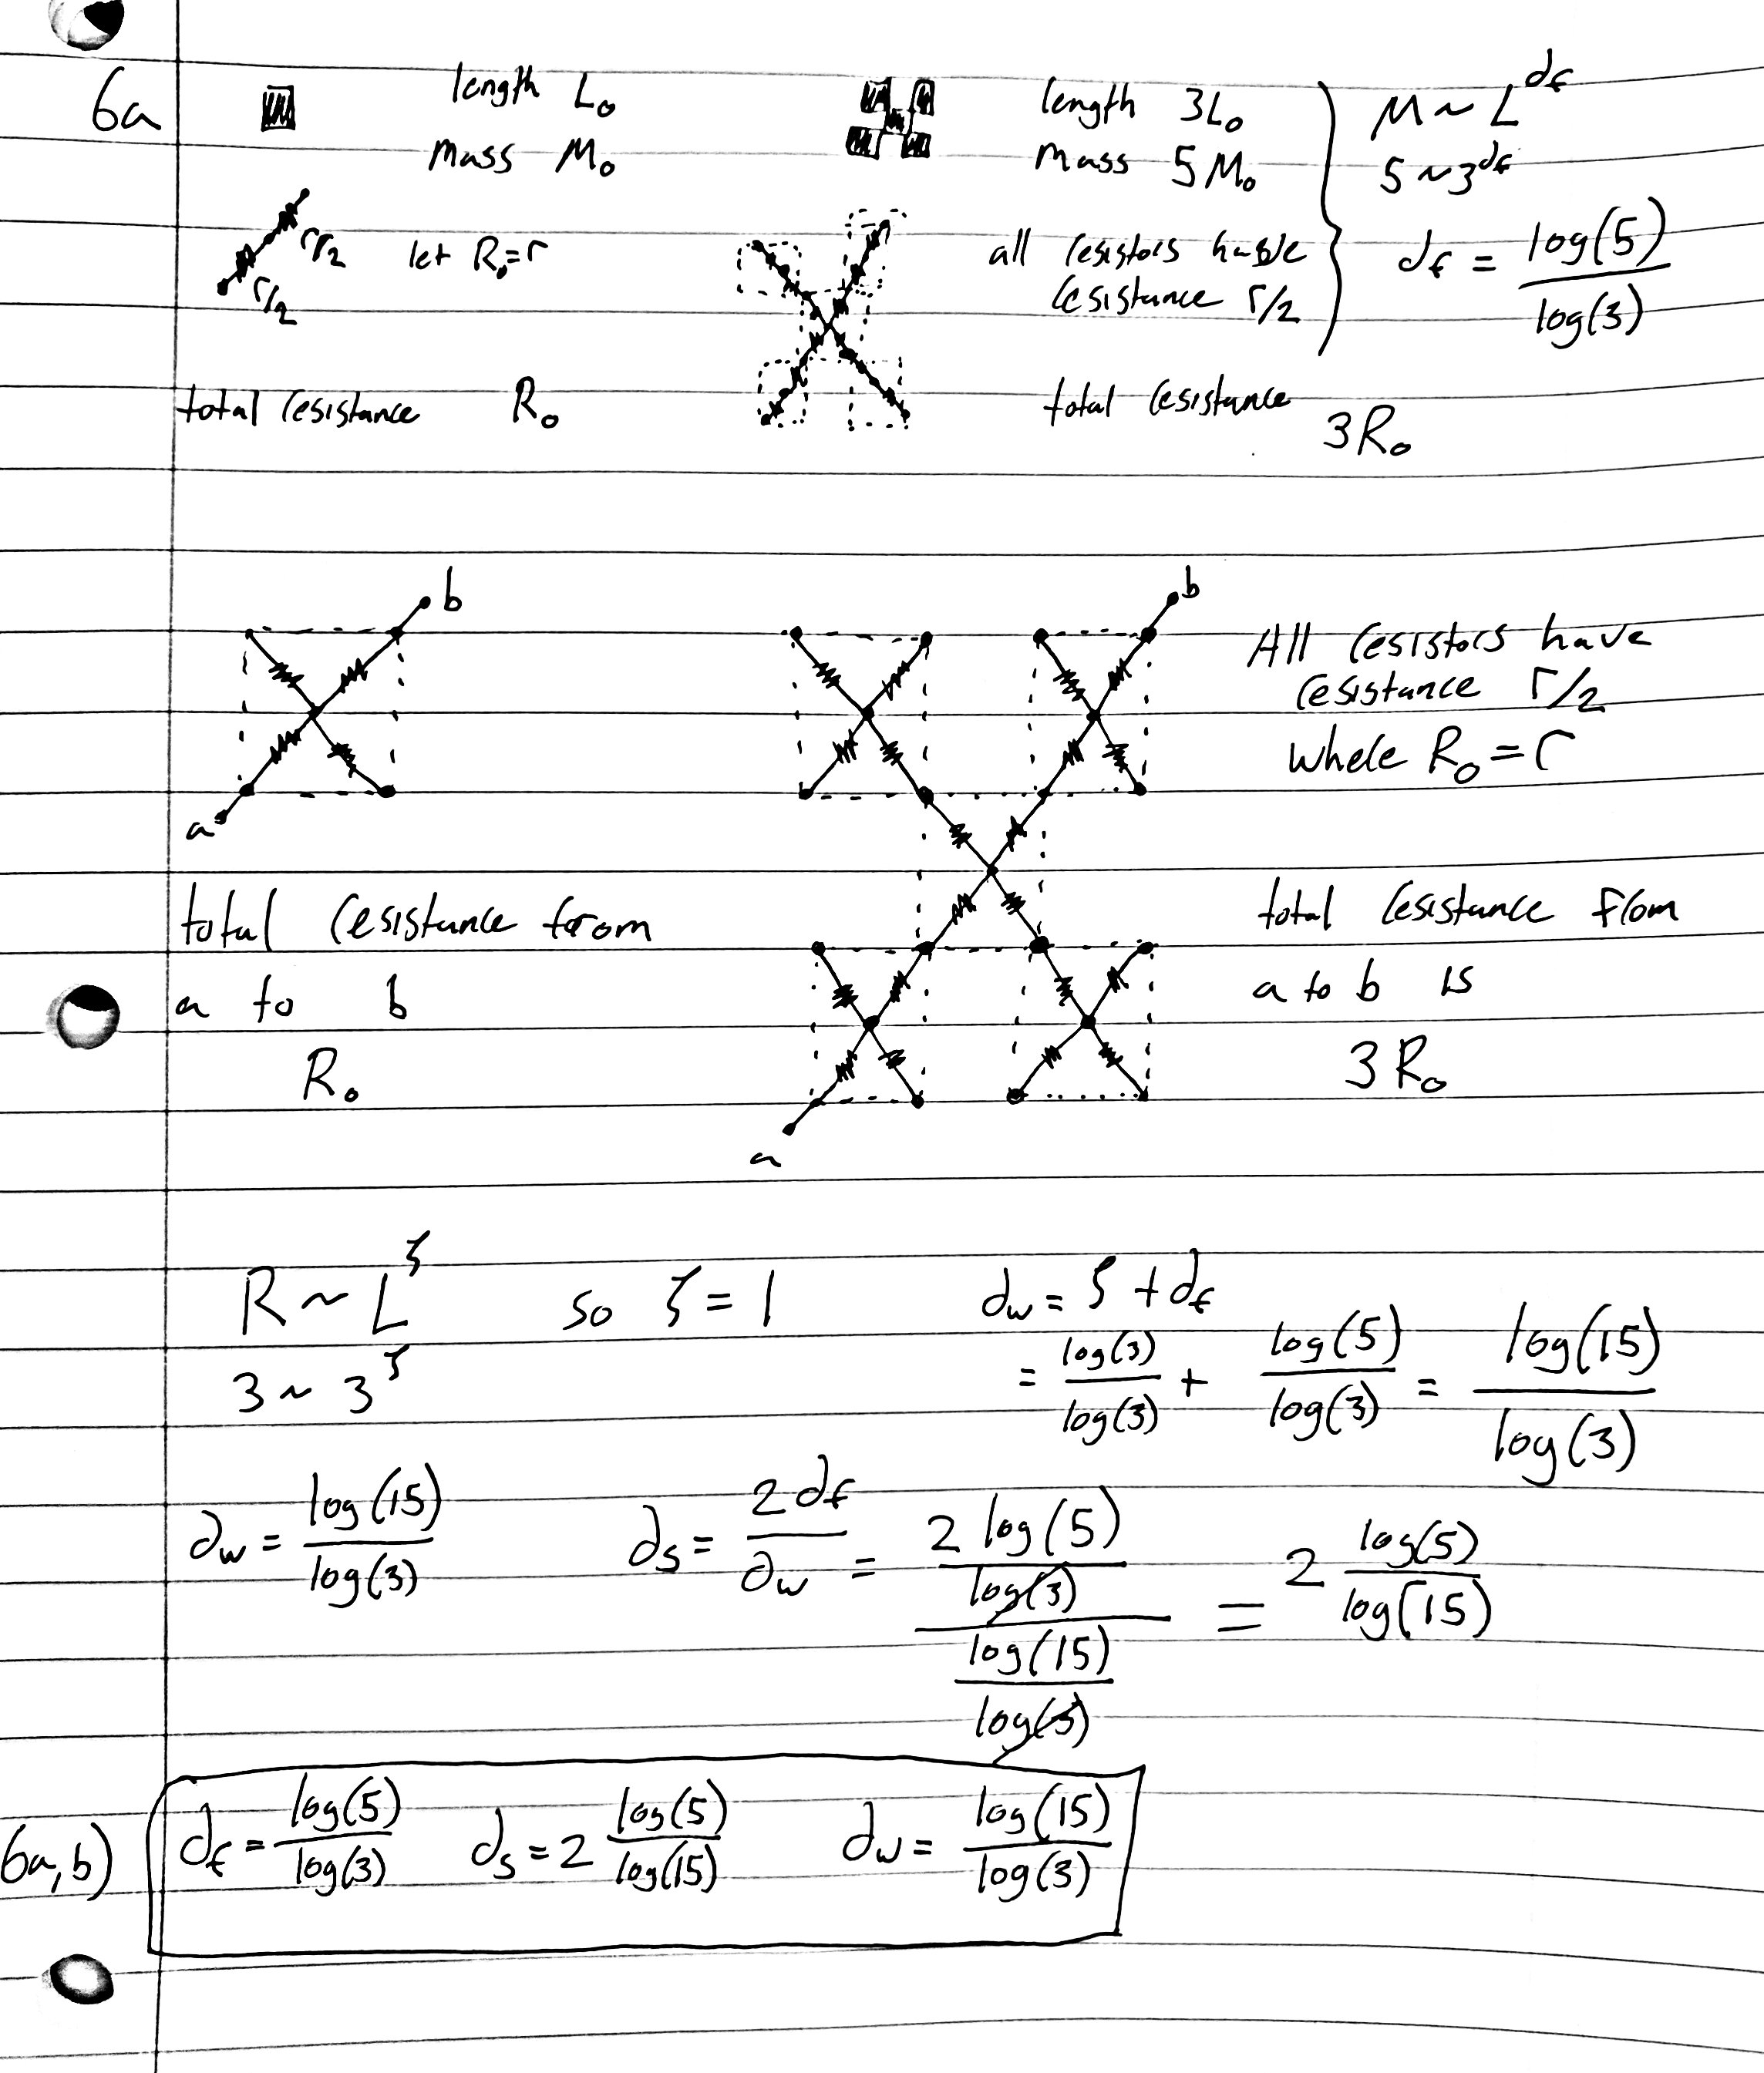
\includegraphics[width=\textwidth]{202211291843391000.jpg}
\end{enumerate}

\end{document}


